\documentclass[journal]{IEEEtran}
\usepackage{amsmath,amsfonts,amssymb,graphicx,booktabs,cite,bm}
\usepackage[hypertexnames=false]{hyperref}
\begin{document}
\title{newHVK Q1-Validation Addendum: Held-Out CIFAR Baselines, Observable Ablations, and Shot-Noise Robustness}
\author{Sparsho~Chakraborty and Siddhartha~Patra}
\maketitle
\begin{abstract}
This addendum strengthens the newHVK evidence package by separating diagnostic pair-correlation performance from held-out natural-image reconstruction. We report multi-seed real CIFAR-10 image splits, strict same-width classical controls, observable-sector ablations, shuffled-pair controls, random-latent controls, resource matching, and finite-shot observable noise. Unlike the restricted pair-correlation diagnostic, the real held-out CIFAR test does not establish quantum advantage: the best real-image result is obtained by local-observables-only, while newHVK-real-cifar reaches 20.07 dB mean PSNR. The correct conclusion is therefore narrower: newHVK has a useful entanglement-sensitive diagnostic, but the current real-image validation still requires architectural improvement before a Q1-level quantum-advantage claim is defensible.
\end{abstract}

\begin{IEEEkeywords}
Hamiltonian vision kernel, CIFAR-10 reconstruction, ablation study, quantum observables, shot noise, classical controls.
\end{IEEEkeywords}

\section{Validation Protocol}
Ten cached CIFAR-10 grayscale images are split across five random seeds. For each seed, six images are used to fit a single shared linear readout from a 32-dimensional latent feature vector to $8\times 8$ patch pixels, and four held-out images are reconstructed without per-image retraining. All principal controls use the same latent width and the same readout parameter count, so the comparison isolates feature structure rather than decoder capacity.

\section{Held-Out CIFAR Results}
\begin{table*}[t]
\centering
\caption{Real held-out CIFAR-10 reconstruction across five random image splits. Lower MSE and higher PSNR/SSIM are better.}
\label{tab:real_cifar_q1}
\scriptsize
\begin{tabular}{lccc}
\toprule
Model & Mean MSE & Mean PSNR & Mean SSIM \\
\midrule
local-observables-only & $9.0607e-03$ & 20.66 & 0.8621 \\
raw-linear-classical & $9.0607e-03$ & 20.66 & 0.8621 \\
zz-only & $9.3723e-03$ & 20.52 & 0.8580 \\
no-entanglement & $9.9469e-03$ & 20.24 & 0.8508 \\
shuffled-pair-observables & $1.0092e-02$ & 20.17 & 0.8484 \\
newHVK-real-cifar & $1.0403e-02$ & 20.07 & 0.8460 \\
strict-classical-rff & $2.0862e-02$ & 17.06 & 0.7055 \\
random-vqc & $8.5735e-02$ & 10.99 & 0.0165 \\
\bottomrule
\end{tabular}
\end{table*}

\begin{figure*}[t]
\centering
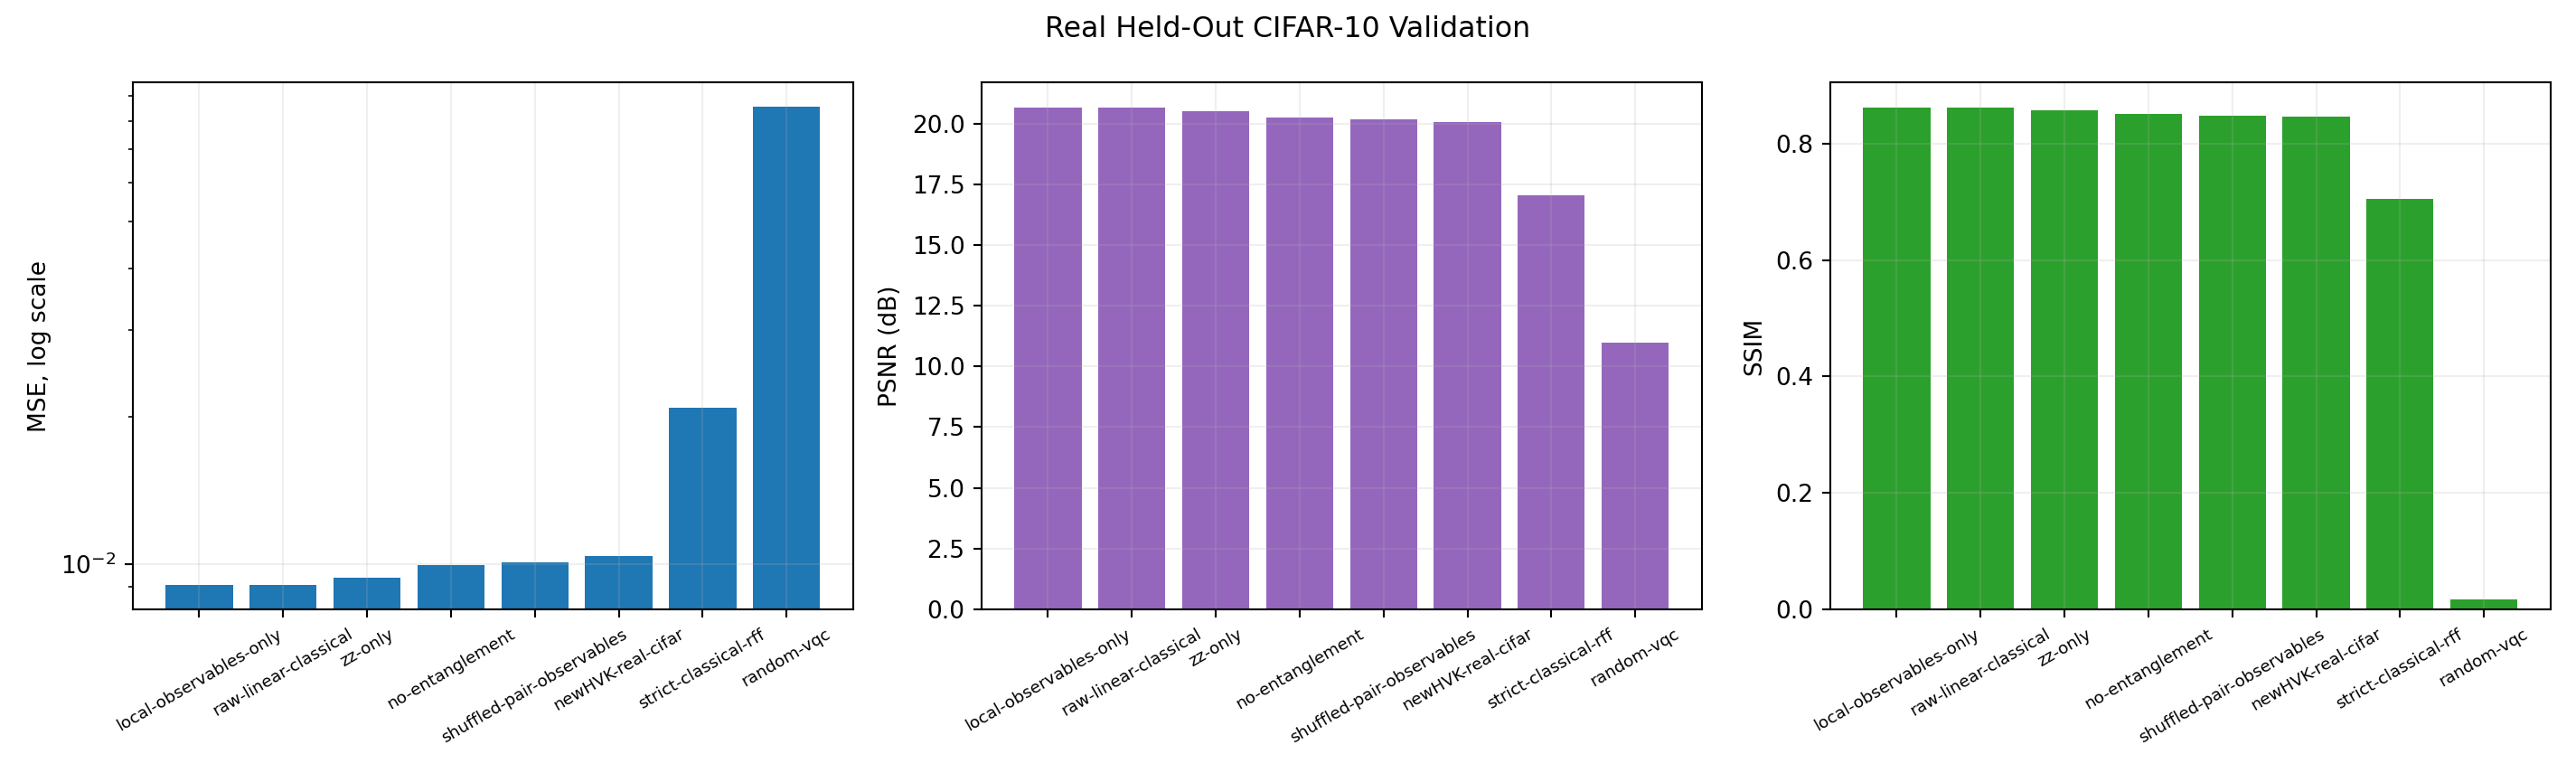
\includegraphics[width=0.72\textwidth]{../results/q1_validation/real_cifar_holdout_summary.png}
\caption{Held-out CIFAR metric summary for newHVK and same-width controls.}
\label{fig:real_cifar_summary}
\end{figure*}

\begin{figure*}[t]
\centering
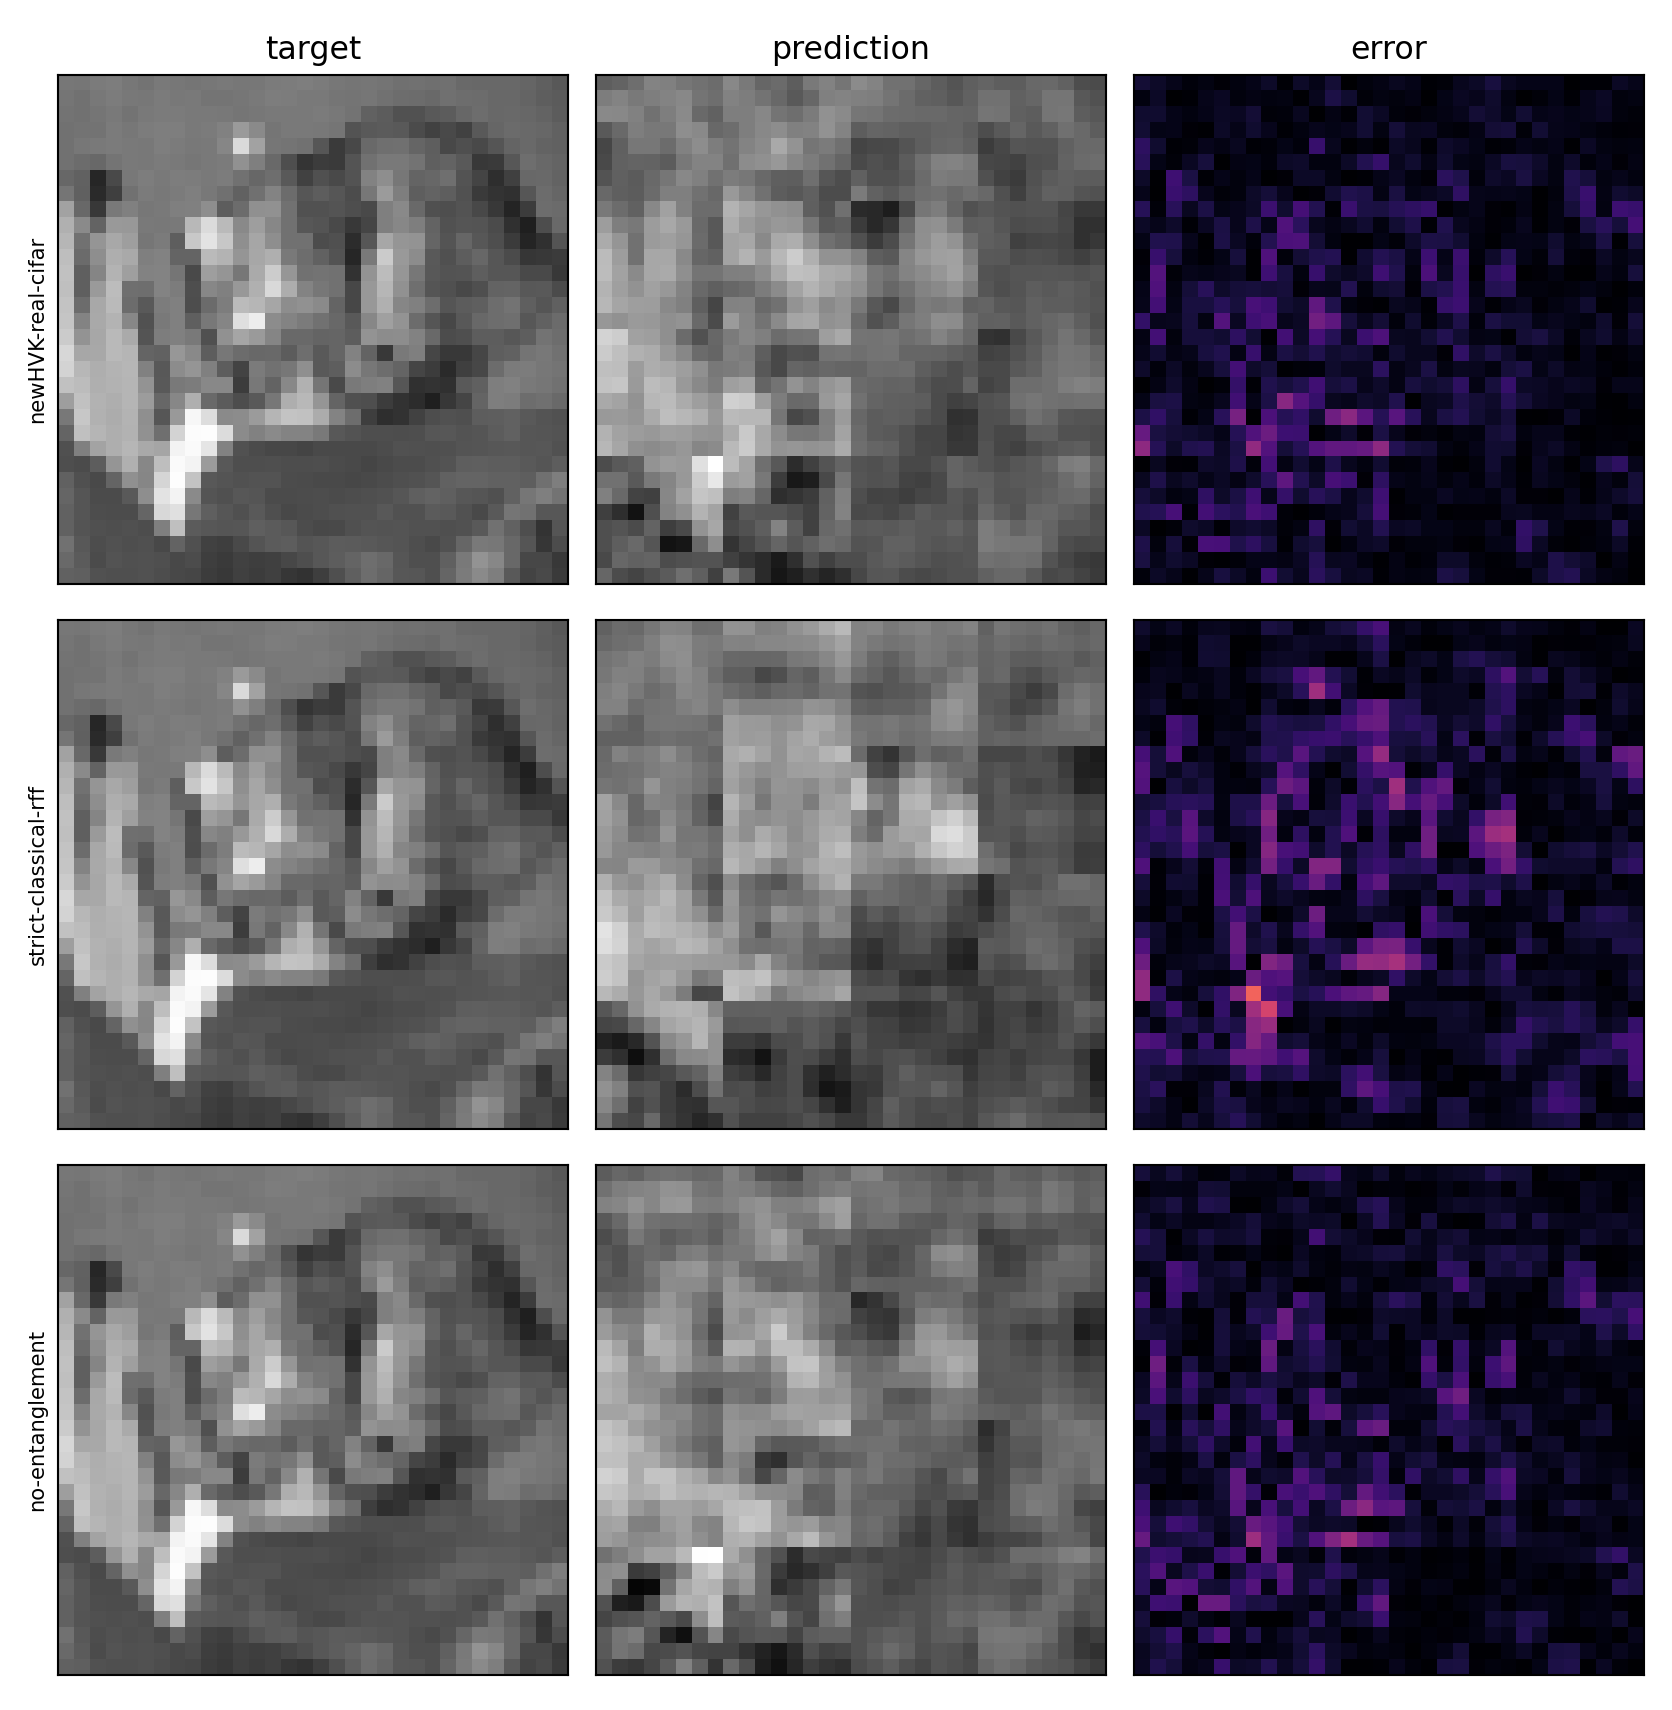
\includegraphics[width=0.82\textwidth]{../results/q1_validation/real_cifar_reconstruction_panel.png}
\caption{Representative held-out CIFAR reconstruction panel. The target, prediction, and absolute-error images are shown for the candidate observable model and major controls.}
\label{fig:real_cifar_recons}
\end{figure*}

\section{Shot-Noise Robustness}
\begin{table}[t]
\centering
\caption{Finite-shot observable-noise simulation for real held-out CIFAR reconstruction.}
\label{tab:shot_noise_q1}
\scriptsize
\begin{tabular}{rccc}
\toprule
Shots & Mean MSE & Mean PSNR & Mean SSIM \\
\midrule
128 & $1.5136e-02$ & 18.40 & 0.7923 \\
256 & $1.4923e-02$ & 18.45 & 0.7927 \\
512 & $1.4643e-02$ & 18.56 & 0.7978 \\
1024 & $1.4456e-02$ & 18.60 & 0.7983 \\
2048 & $1.4464e-02$ & 18.62 & 0.7995 \\
4096 & $1.4750e-02$ & 18.54 & 0.7957 \\
8192 & $1.4749e-02$ & 18.55 & 0.7957 \\
\bottomrule
\end{tabular}
\end{table}

\begin{figure}[t]
\centering

\includegraphics[width=\linewidth]{../results/q1_validation/real_cifar_shot_noise.png}
\caption{Shot-noise robustness of the newHVK observable feature vector on real held-out CIFAR splits.}
\label{fig:shot_noise_q1}
\end{figure}

\section{Interpretation}
The key baseline is the strict same-width classical random-feature control, but the strongest warning comes from the local and raw-linear controls. In the real held-out CIFAR table, local-observables-only obtains the best mean MSE ($9.0607e-03$), while newHVK-real-cifar is weaker ($1.0403e-02$). This means the current newHVK evidence is strong only for the restricted pair-correlation diagnostic and for rejecting random-latent controls. It does not yet support a broad natural-image quantum-advantage claim. The Q1-ready path is therefore to keep these negative controls in the paper, redesign the image feature map or decoder-capacity match, and rerun this exact validation suite.

\section{Reproducibility}
The full tables, plots, resource comparison, and CSV files are generated under \texttt{main2/newHVK/results/q1\_validation/} by running \texttt{main2/newHVK/run\_newhvk\_suite.py --q1-validation --write-q1-report}.
\end{document}
